\section{Materiales y Metodos}
    
    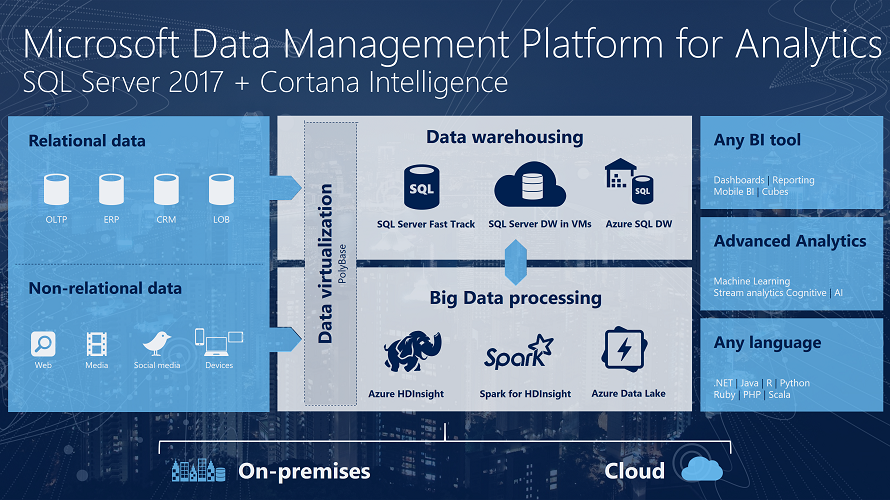
\includegraphics[width=16cm]{imagenes/arquitectura.png}
    
    \begin{enumerate}
        \item \textbf{¿ Por que necesitamos DataLake?}
        \paragraph Las organizaciones que generan valor de negocio exitosamente a partir de sus datos, superarán a sus pares. En una encuesta de Aberdeen, las organizaciones que implementaron un Data Lake superaron a las empresas similares en un 9 porciente en el crecimiento de ingresos orgánicos.\\ \\
        Estos líderes pudieron realizar nuevos tipos de análisis, como el aprendizaje automático a través de nuevas fuentes, como archivos de registro, datos de secuencias de clics, medios sociales y dispositivos conectados a Internet almacenados en el lago de datos. Esto les ayudó a identificar y aprovechar las oportunidades para el crecimiento empresarial más rápido al atraer y retener clientes, aumentar la productividad, mantener dispositivos de forma proactiva y tomar decisiones informadas.\\
        
        \item \textbf{Data Lakes comparado con Data Warehouses: dos enfoques diferentes}
        
        \paragraph Dependiendo de los requisitos, una organización típica requerirá tanto un almacén de datos como un lago de datos, ya que responden a diferentes necesidades y casos de uso.
        \paragraph Un almacén de datos es una base de datos optimizada para analizar datos relacionales provenientes de sistemas transaccionales y aplicaciones de línea de negocios. La estructura de datos y el esquema se definen de antemano para optimizar las consultas SQL rápidas, donde los resultados se utilizan normalmente para informes y análisis operativos. Los datos se limpian, enriquecen y transforman para que puedan actuar como la "fuente única de verdad" en la que los usuarios pueden confiar.
        
    \end{enumerate}
